\documentclass[12,english]{article}
\usepackage[letterpaper, portrait, margin=1in]{geometry}

\usepackage{amsmath}
\usepackage[T1]{fontenc}
\usepackage{babel}
\usepackage{textcomp}
\usepackage{titlesec}
\usepackage{hyperref}
\usepackage{xcolor}
\usepackage{booktabs}
\usepackage{placeins}
\usepackage{graphicx}

\graphicspath{ {img/} }

\hypersetup{
    bookmarks=true,         % show bookmarks bar?
      colorlinks=true,       % false: boxed links; true: colored links
    linkcolor=black,          % color of internal links (change box color with linkbordercolor)
    citecolor=green,        % color of links to bibliography
    filecolor=magenta,      % color of file links
    urlcolor=cyan           % color of external links
}

\begin{document}
\begin{titlepage}
    \begin{center}
        \vspace*{1cm}
        
        \Huge
        \textbf{Module Guide}
        
        \vspace{0.5cm}
        \LARGE
        SFWRENG 3XA3
        
        \vspace{1.5cm}
        
\Large
        Group 30
		\\ Alan Yin (yins1)
		\\ Huajie Zhu (zhuh5)
		\\ Junni Pan (panj10)
        
        \vspace{1.5cm}
        
        \Large
        November 09, 2017
        
    \end{center}
\end{titlepage}

\newpage
\tableofcontents
\listoftables
\listoffigures
\newpage

\section{Major Revision History}
\begin{table}[!htbp]
	\begin{tabular}{|l|l|}
	    \hline
		Date & Revision\\ \hline
		November 6, 2017 & Rough draft of sections\\ \hline
		November 7, 2017 & Revised sections \\ \hline
		November 9, 2017 & Revision 0 complete\\ \hline
		\color{red}{December 6, 2017} & \color{red}{Revision 1 complete}\\ \hline
	\end{tabular}
	\caption{Major Revision History}
\end{table} \color{black}


\section{Introduction}
	\subsection{Overview}
	The Tower Defense game project is a partial re-implementation and refinement based on an existing open source project. The completed project allows the user to build towers on the map to defend enemies from a certain route.
	\subsection{Context}
	The Module Guide (MG) document is an introduction to modules in this project, where the module functionality and specification are created based on Software Requirement Specification (SRS) document. The MG covers all the anticipated and unlikely changes to functional and non-functional requirements specified in SRS, and provids a modular structure for the entire system. The MG also includes the relationship between modules and the corresponding requirements they achieved. At the same time, a Module Interface Specification (MIS) document is also created in the design documents to provide details on every module which are mentioned in MG. 

	\subsection{Design Principles}
	Design Principles being used in this project are Information Hiding and Uses Relation. Information hiding ensures that each module design interface will not change even when the module secret changes.
	

	\subsection{Document Structure}
	
\begin{itemize}

\item Section 1 \newline (Current Section) A brief review of the project and the introduction of Module Guide Document.

\item Section 2 \newline List anticipated and unlikely Changes from Software Requirement Specification document. 

\item Section 3 \newline Give details for the Module Hierarchy, provide the module hierarchy by secrets. 

\item Section 4 \newline Give explanation for the Connection Between Requirements and Design, which shows how the software requirements are accomplished by the listed modules. 

\item Section 5 \newline Provide the Module Decomposition details, including module names, secrets, service or responsibility, and implemented by information for each module listed above. 

\item Section 6 \newline Provide the Traceability Matrices which connect the requirements to the modules, and anticipated changes from Section 2 to the modules. This provides a straightforward representation of how the requirements in SRS are accomplished.

\item Section 7 \newline Provide the Uses Hierarchy for the project, which shows the uses relations between modules.

\item Section 8 \newline Provide the Project Schedule by including up-to-date Gantt chart.

\item Section 9 \newline List the Major Revision History for the document.
\end{itemize}	

\section{Anticipated and Unlikely Changes}

\subsection{Anticipated Changes}

AC1: The game start menu and looking of interface.\\
AC2: The addition of Java gaming library.\\
AC3: The visual representation of tower and critters.\\
AC4: The deletion of map editor feature.\\
AC5: The logic and property of critters and towers for balancing modification.\\
AC6: The addition of AreaAttack tower.\\
AC7: The addition of animation effect and background music.\\
AC8: How wave are grouped into stages with different maps and winning strategies.\\

\subsection{Unlikely Changes}

UC1: Integration of swing and Slick2D windows.\\
UC2: The running environment and devices.\\
UC3: The algorithm for target selection.\\
UC4: The integration of map editor and stage selection option.

\section{Module Hierarchy}

\begin{table}[!htbp]
        \begin{tabular}{ll}
        \toprule
        Level 1 & Level 2 \\
        \midrule
        Hardware Hiding Module & MouseAndKeyboardHandler \\
         \midrule
        Behaviour Hiding Module & Game Module \\
        & GameController Module\\
        & ArtistSwing Module\\
        & Gameclock Module\\ 
		& Critter Module \\
		& Tower Module \\
		& MapTile Module \\
		& Player Module \\
		& GameApplicationFrame Module \\
		& GameState Module \\
		& MainMenu Module \\
		& MenuApplicationFrame Module \\
		
		
		 \midrule
        Software Decision Module & Point Module\\
        & IStrategy Module\\
        & Farthest Module \\
		& Closest Module \\
		& Strongest Module \\
		& Weakest Module \\
		& SetupClass Module \\
		
        \bottomrule
        \end{tabular}
        \caption{Module Hierarchy}
        % Colour for the rulings in tables:
        \makeatletter
           \def\rulecolor#1#{\CT@arc{#1}}
           \def\CT@arc#1#2{%
           \ifdim\baselineskip=\z@\noalign\fi
           {\gdef\CT@arc@{\color#1{#2}}}}
           \let\CT@arc@\relax
          \rulecolor{black!50}
        \makeatother
        \label{Table 1}
        \end{table}

\section{Connection Between Requirements and Design}

The modules are designed into 5 categories, including controllers, helpers, models, strategies, and views. Game module is the main module where the running request is called, and Game Controller module calls every required frames and panels to form the game window. Modules under models category are abstract data types which store the properties of players, towers, critters, maps, etc. These data can be accessed by ArtistSwing module to convert text data into graphical representations, and then the game panels can use graphical representations to display the game to the users on GUI. All the user inputs are done by mouse and keyboard, and they are collected by MouseAndKeyboardHandler module. 

In order to enhance the gameplay experience and to facilitate development process, an external library called slick2D is used in this project. It provides a better way of implementing a clean and unambiguous user interface. Also, buttons, dropdown menus and sliders are included in the game controller window for easier user operation. All the buttons and operation areas are properly sized, and the game window is set in high resolution so that it satisfies the usability requirement. The project can be exported into a jar file. This means it could run on any platform that support Java. It satisfies the requirement where the game is supposed to be cross-platform. The usage of licensed library and open sourced code ensures that the legal requirement is not violated. 


\section{Module Decomposition}
M1: Game Module \newline    
M2: Game Controller Module \newline 
M3: ArtistSwing Module \newline 
M4: Gameclock Module \newline 
M5: MouseAndKeyboardHandler Module \newline 
M6: Critter Module \newline 
M7: Tower Module \newline 
M8: MapTile Module \newline 
M9: Player Module \newline 
M10: Point Module \newline 
M11: Closest Module \newline 
M12: Farthest Module \newline 
M13: IStrategy Module \newline 
M14: Strongest Module \newline 
M15: Weakest Module \newline 
M16: GameApplicationFrame Module \newline 
M17: GameState Module \newline 
M18: MainMenu Module \newline 
M19: MenuApplicationFrame Module \newline 
M20: SetupClass Module \newline 


	\subsection{Game Module}
	\textbf{Secret}: Contents in game panel \\
	\textbf{Services}: This module serves as the initiator of the game project. It starts the application, and sets the resolution to 1000*700. \\
	\textbf{Implemented By}: Java Library
	
	\subsection{Game Controller Module}
	\textbf{Secrets}: Data on map, towers and critters. \\
	\textbf{Services}: Handles all the complex interfacing with map, the towers placed on the map, and critters traversing on shortest path. \\
	\textbf{Implemented By}: Java Library \\
	
	\subsection{ArtistSwing Module}
	\textbf{Secret}: Data on DrawableEntities  \\
	\textbf{Service}: Transform game logic and data into drawable entity information, in order to create graphical representation of game.   \\  
	\textbf{Implemented By}: Java Libraries \\

	\subsection{Gameclock Module}
	\textbf{Secret}: Drawable entity information. \\
	\textbf{Service}: Determine the refresh rate for redrawing entities, and enable pause function for the game project. \\
	\textbf{Implemented By}: Java Libraries\\

	\subsection{MouseAndKeyboardHandler Module}
	\textbf{Secret}: User input \\
	\textbf{Service}: Provide corresponding functions for mouse operations. \\
	\textbf{Implemented By}: Java Libraries\\ 
	
	\subsection{Critter Module}
	\textbf{Secret}: Default setting for every critter. \\
	\textbf{Service}: Abstract data type of a critter object. \\
	\textbf{Implemented By}: Java Libraries\\

    \subsection{Tower Module}
	\textbf{Secret}: Default setting for every tower. \\
	\textbf{Service}: Abstract data type of a tower object.\\
	\textbf{Implemented By}: Java Libraries 
	
	\subsection{MapTile Module}
	\textbf{Secrets}: Usable data from map. \\
	\textbf{Services}: Refers to tiles associated with map.  \\
	\textbf{Implemented By}:  Java Libraries\\
	
	\subsection{Player Module}
	\textbf{Secret}: Player information.  \\
	\textbf{Service}: Abstract data type for player to store player information. \\
	\textbf{Implemented By}: Java Libraries \\
	
	\subsection{Point Module}
	\textbf{Secret}: Usage for points \\
	\textbf{Service}: Simply has an x point, and a y point. Used for positioning  \\ 
	\textbf{Implemented By}: Java Libraries\\
	
	\subsection{Closest Module}
	\textbf{Secret}: Tower information \\
	\textbf{Service}: Finds the target based on who is closest.  \\ 
	\textbf{Implemented By}: Java Libraries\\
	
	\subsection{Farthest Module}
	\textbf{Secret}: Tower information \\
	\textbf{Service}: Finds the target based on who is farthest. \\ 
	\textbf{Implemented By}: Java Libraries\\
	
    \subsection{IStrategy Module}
	\textbf{Secret}: Algorithm details \\
	\textbf{Service}:  Find a target critter.  \\ 
	\textbf{Implemented By}: Java Libraries\\
	
	\subsection{Strongest Module}
	\textbf{Secret}: Tower information \\
	\textbf{Service}:  Finds the target based on who is strongest.  \\ 
	\textbf{Implemented By}: Java Libraries\\
	
	\subsection{Weakest Module}
	\textbf{Secret}: Tower information \\
	\textbf{Service}:  Finds the target based on who is weakest.  \\ 
	\textbf{Implemented By}: Java Libraries\\
	
	\subsection{GameApplicationFrame Module}
	\textbf{Secret}: Detailed data in the frame. \\
	\textbf{Service}: Swing implementation of game window.  \\ 
	\textbf{Implemented By}: Swing\\
	
	\subsection{GameState Module}
	\textbf{Secret}: Data in game states. \\
	\textbf{Service}: Transition from main menu to game application.  \\ 
	\textbf{Implemented By}: Slick2D\\
	
	\subsection{MainMenu Module}
	\textbf{Secret}: Contents in main menu. \\
	\textbf{Service}: Slick2D main menu setup.  \\ 
	\textbf{Implemented By}: Slick2D\\
	
	\subsection{MenuApplicationFrame Module}
	\textbf{Secret}: contents in menu. \\
	\textbf{Service}: Set default map and all button application.  \\ 
	\textbf{Implemented By}: Slick2D\\
	
	\subsection{SetupClass Module}
	\textbf{Secret}: Data from Slick2D window. \\
	\textbf{Service}: Create link between main menu and game application.  \\ 
	\textbf{Implemented By}: Slick2D\\
	
	
\section{Traceability Matrices}

\subsection{Modules and Requirements}

\begin{table}[!htbp]
      \begin{tabular}{ll}
        \toprule
        Requirement & Modules \\
        \midrule
        \multicolumn{2}{c}{Functional Requirements} \\
        \midrule
        FR1 & M16, M17, M18, M19, M20 \\
        FR2 & M3, M6, M7, M8 \\
        FR3 & M3, M7, M10, M16 \\
        FR4 & M2, M9, M17, M18, M19 \\
        
        \midrule
        \multicolumn{2}{c}{Non-functional Requirements} \\
        \midrule
        NF1 & M17, M18, M19 \\
        NF2 & M16 \\
        NF3 & M1 \\
        NF4 & M2, M4 \\
        NF5 & M17 \\
        NF6 & M1 \\
        NF7 & M1, M3 \\
        NF8 & M1-M20 \\
        NF9 & M17, M18, M19, M20 \\
        
        \bottomrule
        \end{tabular}
        \caption{Trace Between Requirements and Modules}
        % Colour for the rulings in tables:
        \makeatletter
           \def\rulecolor#1#{\CT@arc{#1}}
           \def\CT@arc#1#2{%
           \ifdim\baselineskip=\z@\noalign\fi
           {\gdef\CT@arc@{\color#1{#2}}}}
           \let\CT@arc@\relax
          \rulecolor{black!50}
        \makeatother
        \label{Table 2}
        \end{table}


\subsection{Modules and Anticipated Changes}
    
        \begin{table}[!htbp]
        \begin{tabular}{ll}
        \toprule
        Anticipated Changes & Modules \\
        \midrule
        AC1 & M1, M17, M18, M19, M20\\
        AC2 & M17, M18, M19, M20\\
        AC3 & M3, M6, M7\\
        AC4 & M2\\
        AC5 & M7, M8\\
        AC6 & M7, M8\\
        AC7 & M17, M18\\
        AC8 & M17\\
    
        \bottomrule
        \end{tabular}
        \caption{Trace Between Requirements and Modules}
        % Colour for the rulings in tables:
        \makeatletter
           \def\rulecolor#1#{\CT@arc{#1}}
           \def\CT@arc#1#2{%
           \ifdim\baselineskip=\z@\noalign\fi
           {\gdef\CT@arc@{\color#1{#2}}}}
           \let\CT@arc@\relax
          \rulecolor{black!50}
        \makeatother
        \label{Table 3}
        \end{table}

\FloatBarrier
\section{Uses Hierarchy Between Modules}

\begin{figure}[h]
\centering
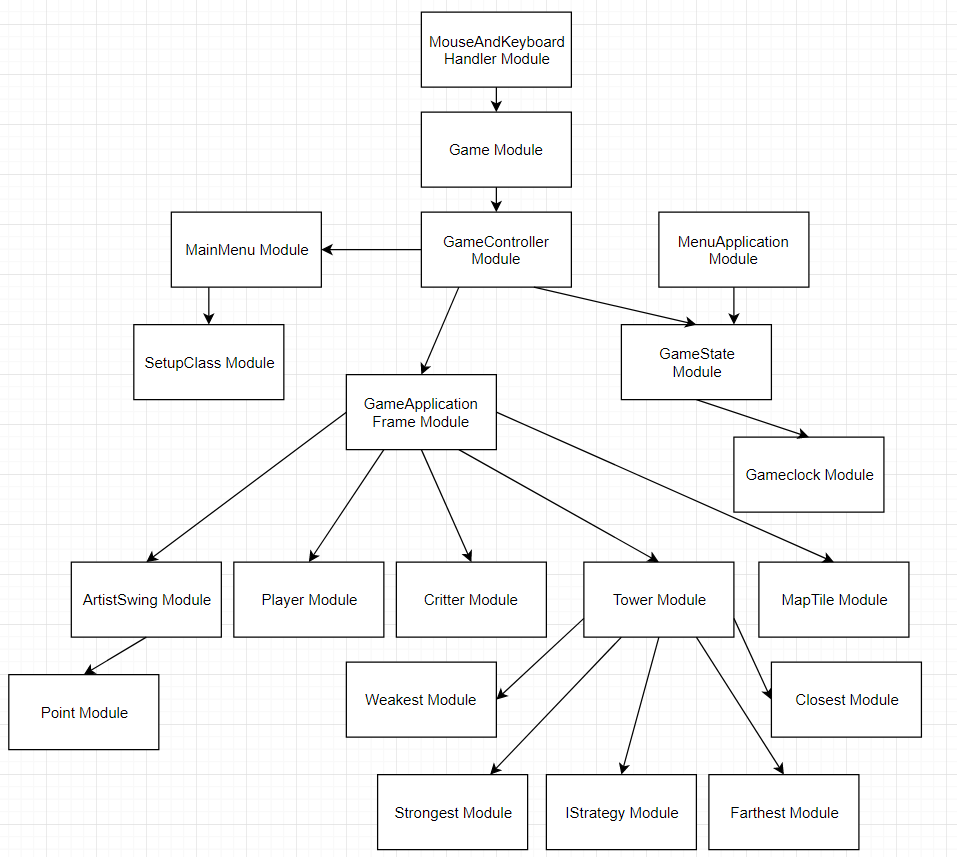
\includegraphics[width=0.7\textwidth]{hierarchy.png}
\caption{Uses hierarchy between modules}
\end{figure}

\clearpage

\section{Schedule}

\subsection{Gantt}
    \begin{figure}[h]
    \centering
	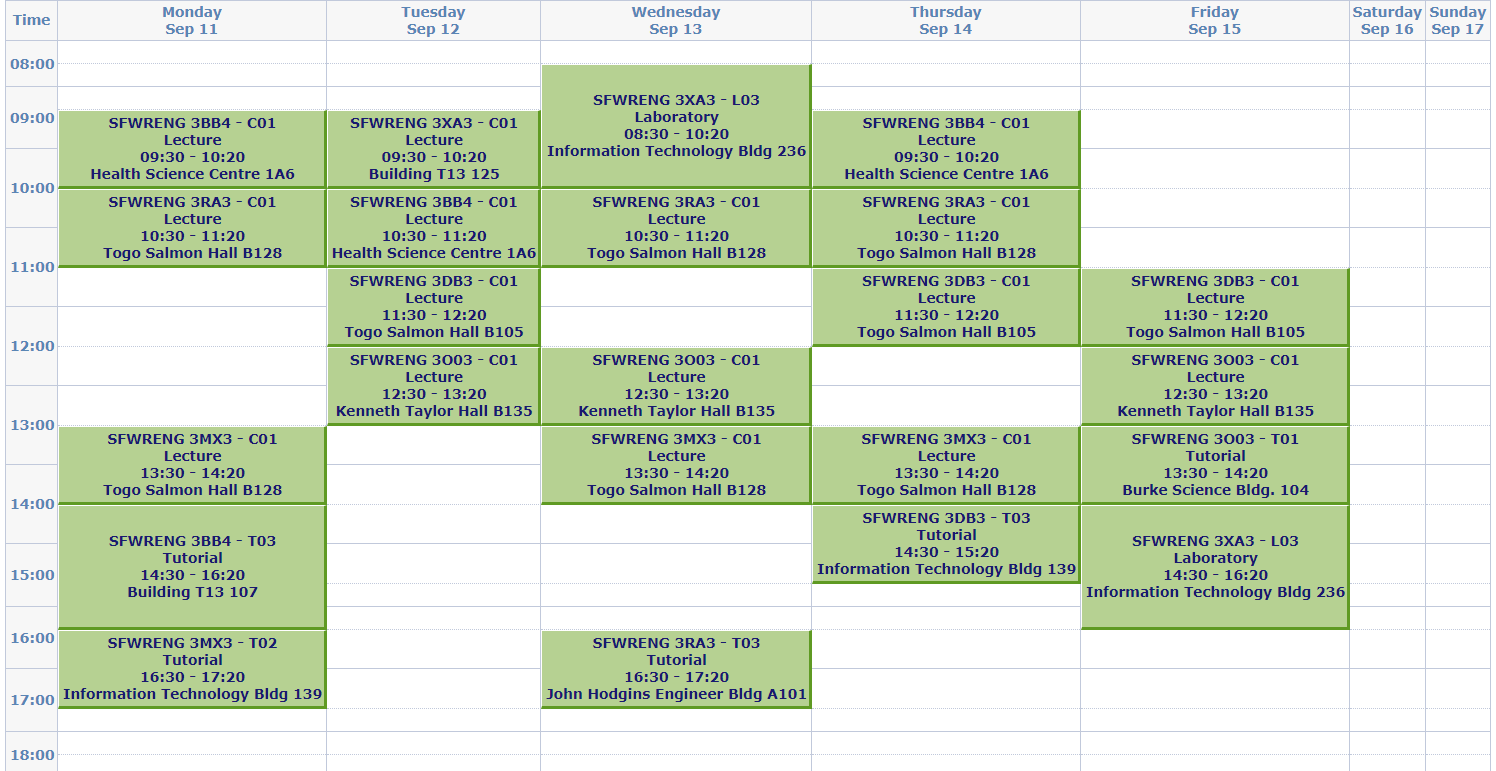
\includegraphics[width=1.1\textwidth]{gantt.png}
    \caption{Gantt chart of project schedule}
	\end{figure}

	\begin{figure}[h]
	\centering
	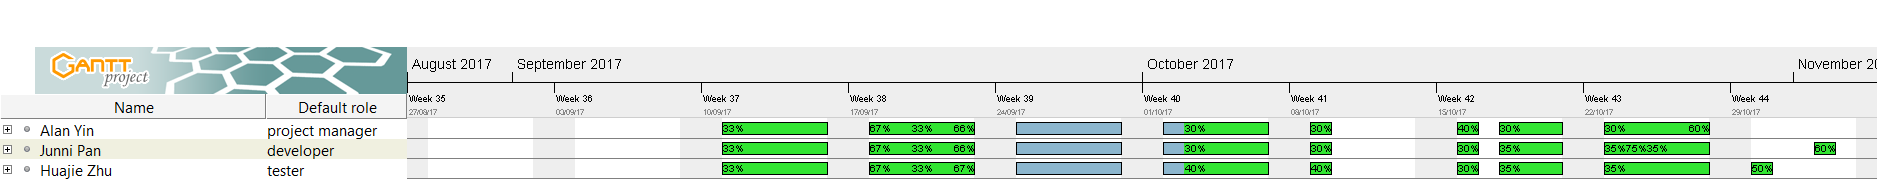
\includegraphics[width=1\textwidth]{resource.png}
	\caption{Gantt chart(resources) of project schedule}
	\end{figure}
	



\end{document}
